\documentclass[a4]{scrartcl}

\usepackage{graphicx}
%\usepackage{mathptmx}      % use Times fonts if available on your TeX system
\usepackage{multicol}
\usepackage{multirow}

% Eigene Defs
\usepackage{amsmath,amsfonts,amssymb}
\usepackage{xspace}
\usepackage{intmacros}
\usepackage{subfigure}
\usepackage[algoruled]{algorithm2e}
\usepackage{tikz}
\newcommand*\circled[1]{%
  \tikz[baseline=(C.base)]\node[draw,circle,inner sep=0.3pt](C){#1};
  \hspace{-1.3ex}
}
\newcommand{\iv}[2]{\ensuremath{[#1, #2]}\xspace}
\newcommand{\aff}[1]{\ensuremath{\hat{#1}}\xspace}
\def\wlst{\ensuremath{\mathcal{L}}\xspace}
\def\flst{\ensuremath{\mathcal{L_\mathrm{final}}}\xspace}
\def\den{\ensuremath{\bfm{\Phi}}\xspace}
\newcommand{\pow}[0]{\ensuremath{\mathrm{pow}}\xspace}
%\newcommand{\rad}[0]{\ensuremath{\mathrm{pow}}\xspace}
\graphicspath{{./figures/}}

\newcommand{\yalaa}{\texttt{YalAA}\xspace}

\author{Stefan Kiel}
\title{yalaa - Yet Another Library for Affine Arithmetic}
\subtitle{Implementation Manual}
\date{\today}

\begin{document}

\maketitle

\section{Introduction}
\label{sec:overview}
.....\\
As a template library, \yalaa is usable with arbitrary (arithmetic) base
types. However, only a specialization for the IEEE754 double is currently
provided and discussion in the following sections.

\section{Preliminaries}
\label{sec:preliminaries}

\subsection{Interval Arithmetic}
\label{sec:interval-arithmetic}

\subsection{Affine Arithmetic}
\label{sec:affine-arithmetic}

\section{Affine Approximations}
\label{sec:affine-appr}
We can not carry out a non affine operation or function directly on affine
forms. However, it is possible to use an affine approximation and bound the
(non-linear) approximation error with an error term. Methods for calculating
affine approximations are outlined and discussed in \cite{stolfi1997} by de
Figueiredo and Stolfi. Following them, we will also limit ourselves to affine
approximations of the form
\[
f^a(\epsilon_1,...,\epsilon_n) = \alpha \aff x + \beta \aff y + \zeta
\]
for the two input forms $\aff x, \aff y$. Two methods for deriving such
approximations are discussed there: The Chebyshev optimal affine approximation
and the min-range approximation. Both methods are only suitable for functions
which are strictly convex or concave over the considered domain. The latter is
implemented in \yalaa for those functions. For functions not satisfying these
condition a Taylor series expansion is used, as described in
Sect. \ref{sec:taylor-series}.


\section{Implementation}
\label{sec:implementation}

\subsection{Important Classes}
\label{sec:non-concept-classes}
In this section the most important classes of \yalaa are described. Concepts
are described in Sect. \ref{sec:concepts}.

\paragraph{AffineForm}

\texttt{AffineForm} combines the several policy classes and concepts to a
working object-oriented arithmetic type. It offers the usual operators and the
elementary functions (Tab. \ref{tab:affine_form}). As a template class the
function can be widely customized. The declaration is as follows:
\begin{tiny}
\begin{verbatim}
template<typename T, \
         template<typename> class ET, \
         template<typename, template<typename> class> class AC, \
         template<typename, template<typename> class, template<typename, template<typename> class> class, class> class AR, \
         template<typename, template<typename> class, template<typename, template<typename> class> class> class AP, \
         typename EP, \
         typename IV>
class AffineForm { ... };
\end{verbatim}
\end{tiny}
The base type \texttt{T} is used for representing the
partial deviations. \texttt{AffineForm} makes no assumptions about this type,
but you have to provide a specialization of the \texttt{base\_traits} template
for a custom type. Further the interval type \texttt{IV} and \texttt{T} have
to fit into one another. A specialization of \texttt{base\_traits} is required for
\texttt{IV} also. The template parameters \texttt{ET, AC, AR, AP} are also templates, but
\emph{their} template parameters are automatically determined through template
template parameters. They model the concepts \texttt{ErrorTerm},
\texttt{AffineCombination}, \texttt{AffinePolicy} and \texttt{ErrorPolicy}
described in Sect. \ref{sec:concepts}.

\paragraph{ArithmeticError}
\label{sec:arithmeticerror}
\begin{figure}[h]
  \centering
  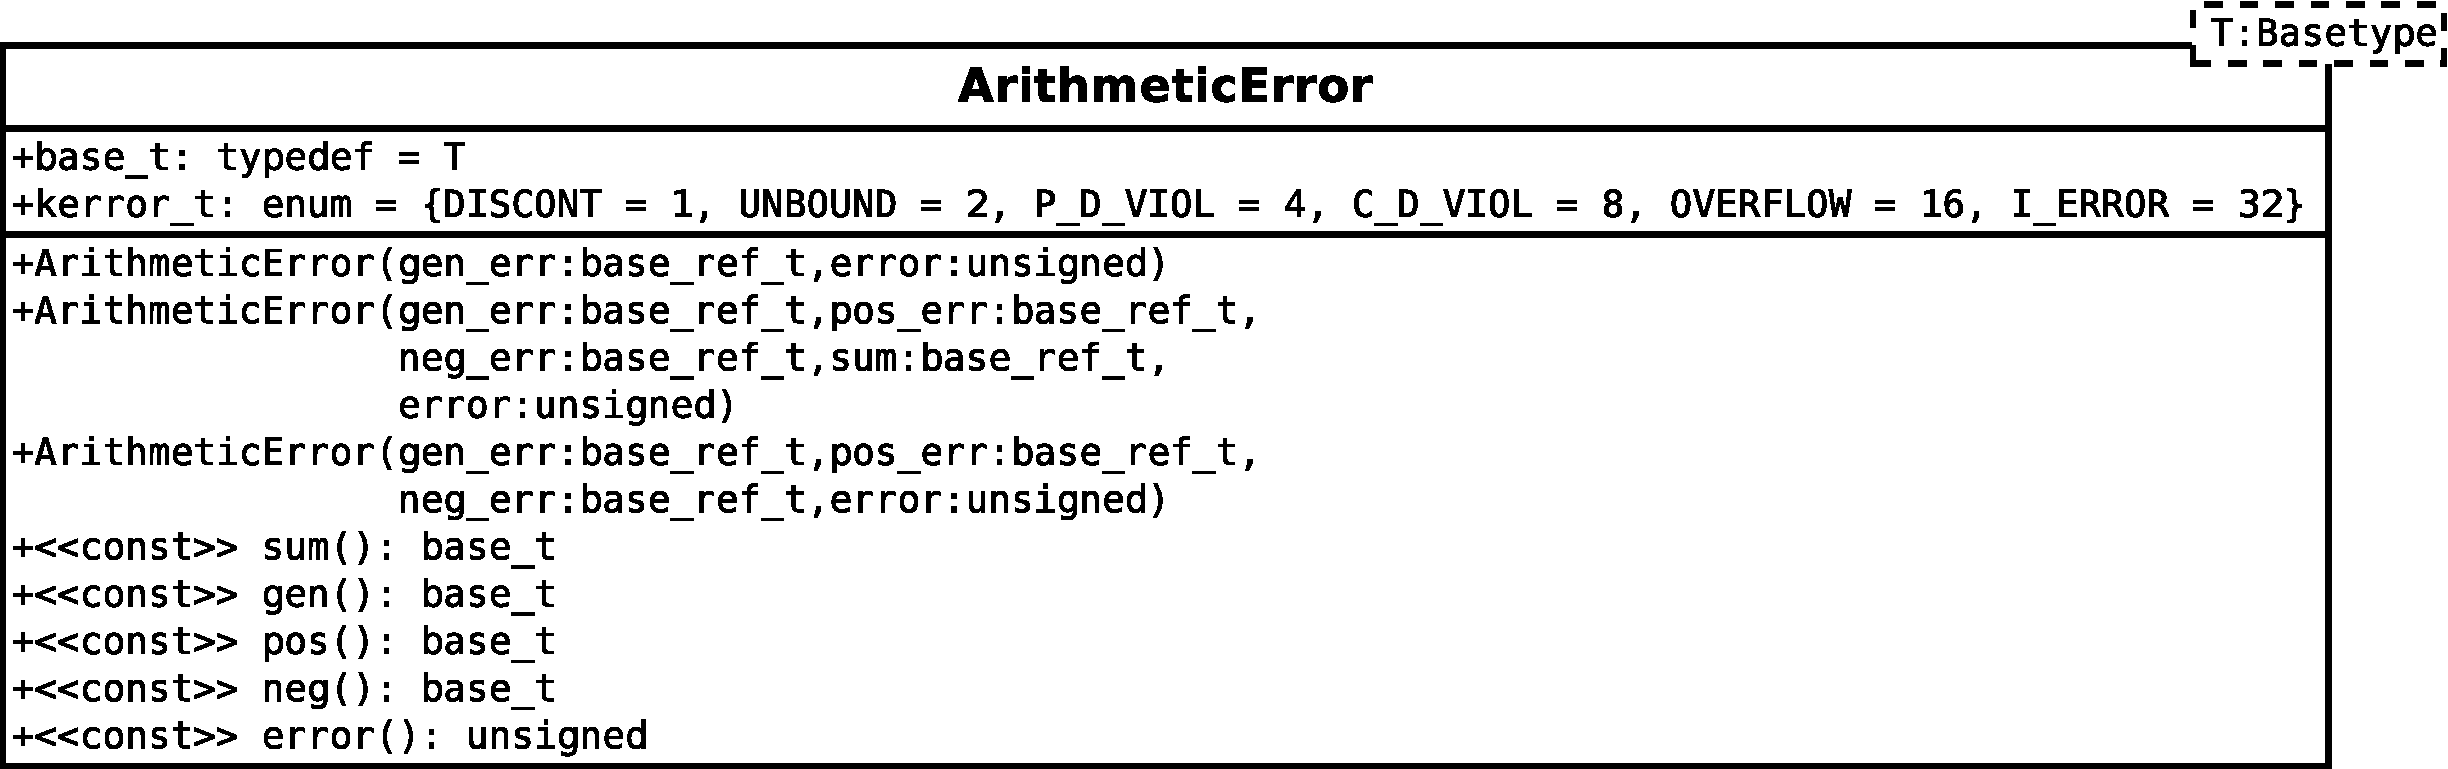
\includegraphics[width=0.9\textwidth]{arithmeticerror}
  \caption{\texttt{ArithmeticError} class}
  \label{fig:arithmeticerror}
\end{figure}
The \texttt{ArithmeticError} class is responsible for handling rounding
errors and approximation errors. Further it stores information about
computational errors \emph{inside} the \texttt{ArithmeticKernel}. An overview
of its operations is given in Fig. \ref{fig:arithmeticerror}.

Rounding and approximations errors are split into three groups:
\emph{general}, \emph{positive} and \emph{negative}. General errors are
identically to the standard error term model where $\epsilon_i$ is assumed to
lie in the interval $\iv{-1}{1}$. The latter two can combined with noise
variables lying inside $\iv{0}{1}$ and $\iv{-1}{0}$
(cf. \cite{messine2002}). However, it's up to the concrete
\texttt{ArithmeticKernel} whether it provides the extended model and up to the
\texttt{AffinePolicy} how it maps the different error types. Obviously the
both new terms can also combined with a standard $\epsilon_i$. This enlarges
the enclosures but nevertheless provides a valid bound. The errors are
accessed through the \texttt{gen}, \texttt{pos}, \texttt{neg} functions. If
only the sum is needed, it can retrieved with the \texttt{sum} function.

Further \texttt{ArithmeticError} defines the \texttt{kerror\_t} type defining
a minimum set of errors that every kernel should propagate: 
\begin{description}
\item[\texttt{DISCONT}] Function is discontinuous
\item[\texttt{UNBOUND}] Result has no finite bounds
\item[\texttt{P\_D\_VIOL}] Partial violation of natural domain
\item[\texttt{C\_D\_VIOL}] Complete violation of natural domain
\item[\texttt{OVERFLOW}] Overflow 
\item[\texttt{ERROR}] Unknown error
\end{description}
The \texttt{DISCONT} error indicates that the operation is discontinuous over
the affine form.  An error of type \texttt{UNBOUNDED} is raised if the result
of the operation is unbounded\footnote{As affine forms cannot represent
  improper intervals like $[x, \infty)$, the \texttt{UNBOUNDED} flag is raised
  in this case.} By contrast \texttt{OVERFLOW} is used for indicating that the
result is bounded but can not represented with used types. The
\texttt{P\_D\_VIOL} indicates that a function was called with an argument
lying partially outside its natural domain. For example let $\aff x = 0 +
2\epsilon_1$. Its range is $\x = \iv{-2}{2}$. Then we can still evaluate
$\sqrt{\aff x}$, but the negative parts of its range are ignored and
\texttt{P\_D\_VIOL} is raised. If we modify our example and choose $\aff x =
-2 + -1 \epsilon_1$ with $\x = \iv{-3}{-1}$, $\sqrt{\aff x}$ will raise
\texttt{C\_D\_VIOL} as the whole affine form lies outside of the square root's
natural domain.  or an overflow occurred. The last flag indicates a general
error inside the kernel.  Raised error flags can determined through the
\texttt{error()} function, which returns an appropriate bitmask.

An \texttt{ArithmeticKernel} should support at least these flags. Otherwise
error policies are not able to work correctly. It's up to the kernel to
provide additional informations through extra flags. However, in this case a
custom \texttt{ErrorPolicy} tightly coupled with the kernel is necessary for
exploiting them.

\subsection{Concepts}
\label{sec:concepts}
\yalaa is a template library and can customized with policy
classes\footnote{See \cite{...} for more information on policy-based
  design.}. It is possible to exchange policy classes in order to alter
\yalaa's behavior. Policy classes do not have common base classes. Nonetheless
they are sort of polymorphic, often called \emph{static} or
\emph{compile-time} polymorphism. They achieve this by following a
\emph{concept}: An interface with a common set of \texttt{static} functions
and \emph{typedef}'s. In contrast to
runtime-polymorphism there is currently no formal support for defining
concept's in C++. So it's up to the programmer to follow the concepts or to
face awful template related error messages ;-).

\paragraph{ErrorTerm}
\label{sec:errorterm}
\begin{figure}[h]
  \centering
  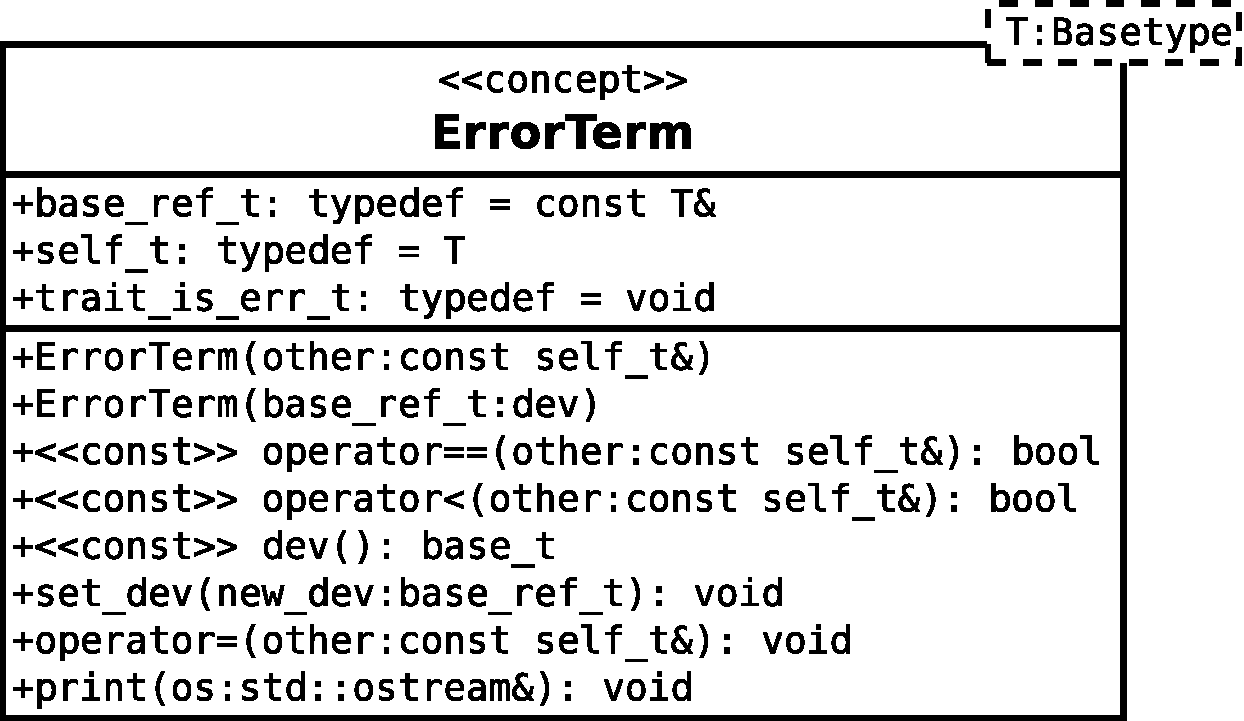
\includegraphics[width=0.4\textwidth]{errorterm}
  \caption{Concept defining an ErrorTerm}
  \label{fig:error_term}
\end{figure}
An error term $\epsilon_i x_i$ is a combination of a symbolic noise variable
$\epsilon_i$ and a partial deviation $x_i$. The partial deviation's type
determines the base type of the affine form. While the concrete type of the
$\epsilon$'s is implementation defined, it is necessary to define an ordering
on them. If the constructor is called, the error term is responsible for
acquiring a new previously unused noise symbol.  The rest of the concept is
straightforward, see Fig. \ref{fig:error_term} for a complete overview. 

\paragraph{AffineCombination}
\label{sec:affinecombination}
\begin{figure}[h]
  \centering
  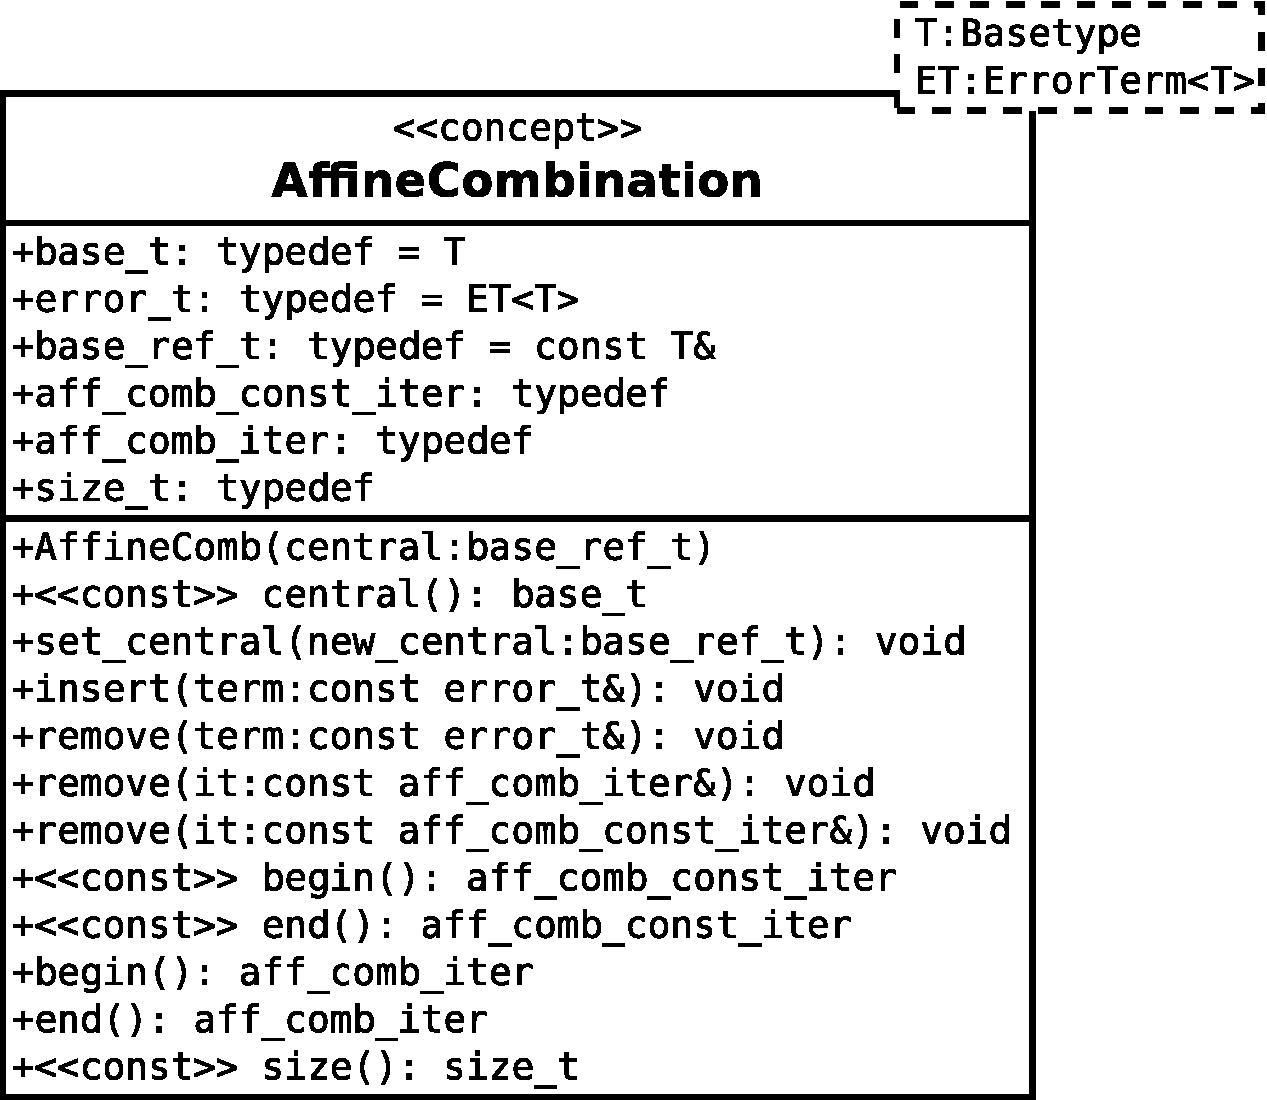
\includegraphics[width=0.4\textwidth]{affinecombination}
  \caption{Concept defining an AffineCombination}
  \label{fig:affine_comb}
\end{figure}
This concept represents an affine combination $x_1\epsilon_i + \cdots +
x_n\epsilon_n$ of error terms and a central value $x_0$ not associated with a
symbolic noise variable. The iterators have to respect the ordering defined by
the error terms. For the full concept cf. Fig. \ref{fig:affine_comb}. 

\paragraph{Affine operations}
\label{sec:affine-operations}
Affine operations are not a template class but a bunch of free functions which
can work on classes fulfilling the \texttt{AffineCombination} concept. A valid
implementation has to provide functions with the following signatures:
\begin{verbatim}
template<typename AC>
unsigned mul_ac_s(AC* ac, typename AC::base_ref_t s);

template<typename AC>
unsigned add_ac_s(AC* ac, typename AC::base_ref_t s);

template<typename AC>
unsigned neg_ac(AC* ac);

template<typename AC, bool CENTRAL = true>
unsigned add_ac_ac(AC* ac1, const AC& ac2);

template<typename AC, bool CENTRAL = true>
unsigned sub_ac_ac(AC* ac1, const AC& ac2); 
\end{verbatim}
providing the usual affine operations. These consist of scaling
(\texttt{mul\_ac\_s}) with a scalar of type \texttt{T::base\_ref\_t}, adding a
scalar (\texttt{add\_ac\_s}) and negate an entire form. Further adding
(\texttt{add\_ac\_ac}) and subtracting (\texttt{sub\_ac\_ac}) two affine
combinations has to be supported. The result is always stored in the first
affine combination supplied as argument.

\paragraph{ArithmeticKernel}
\label{sec:arithmetickernel}
\begin{figure}[h]
  \centering
  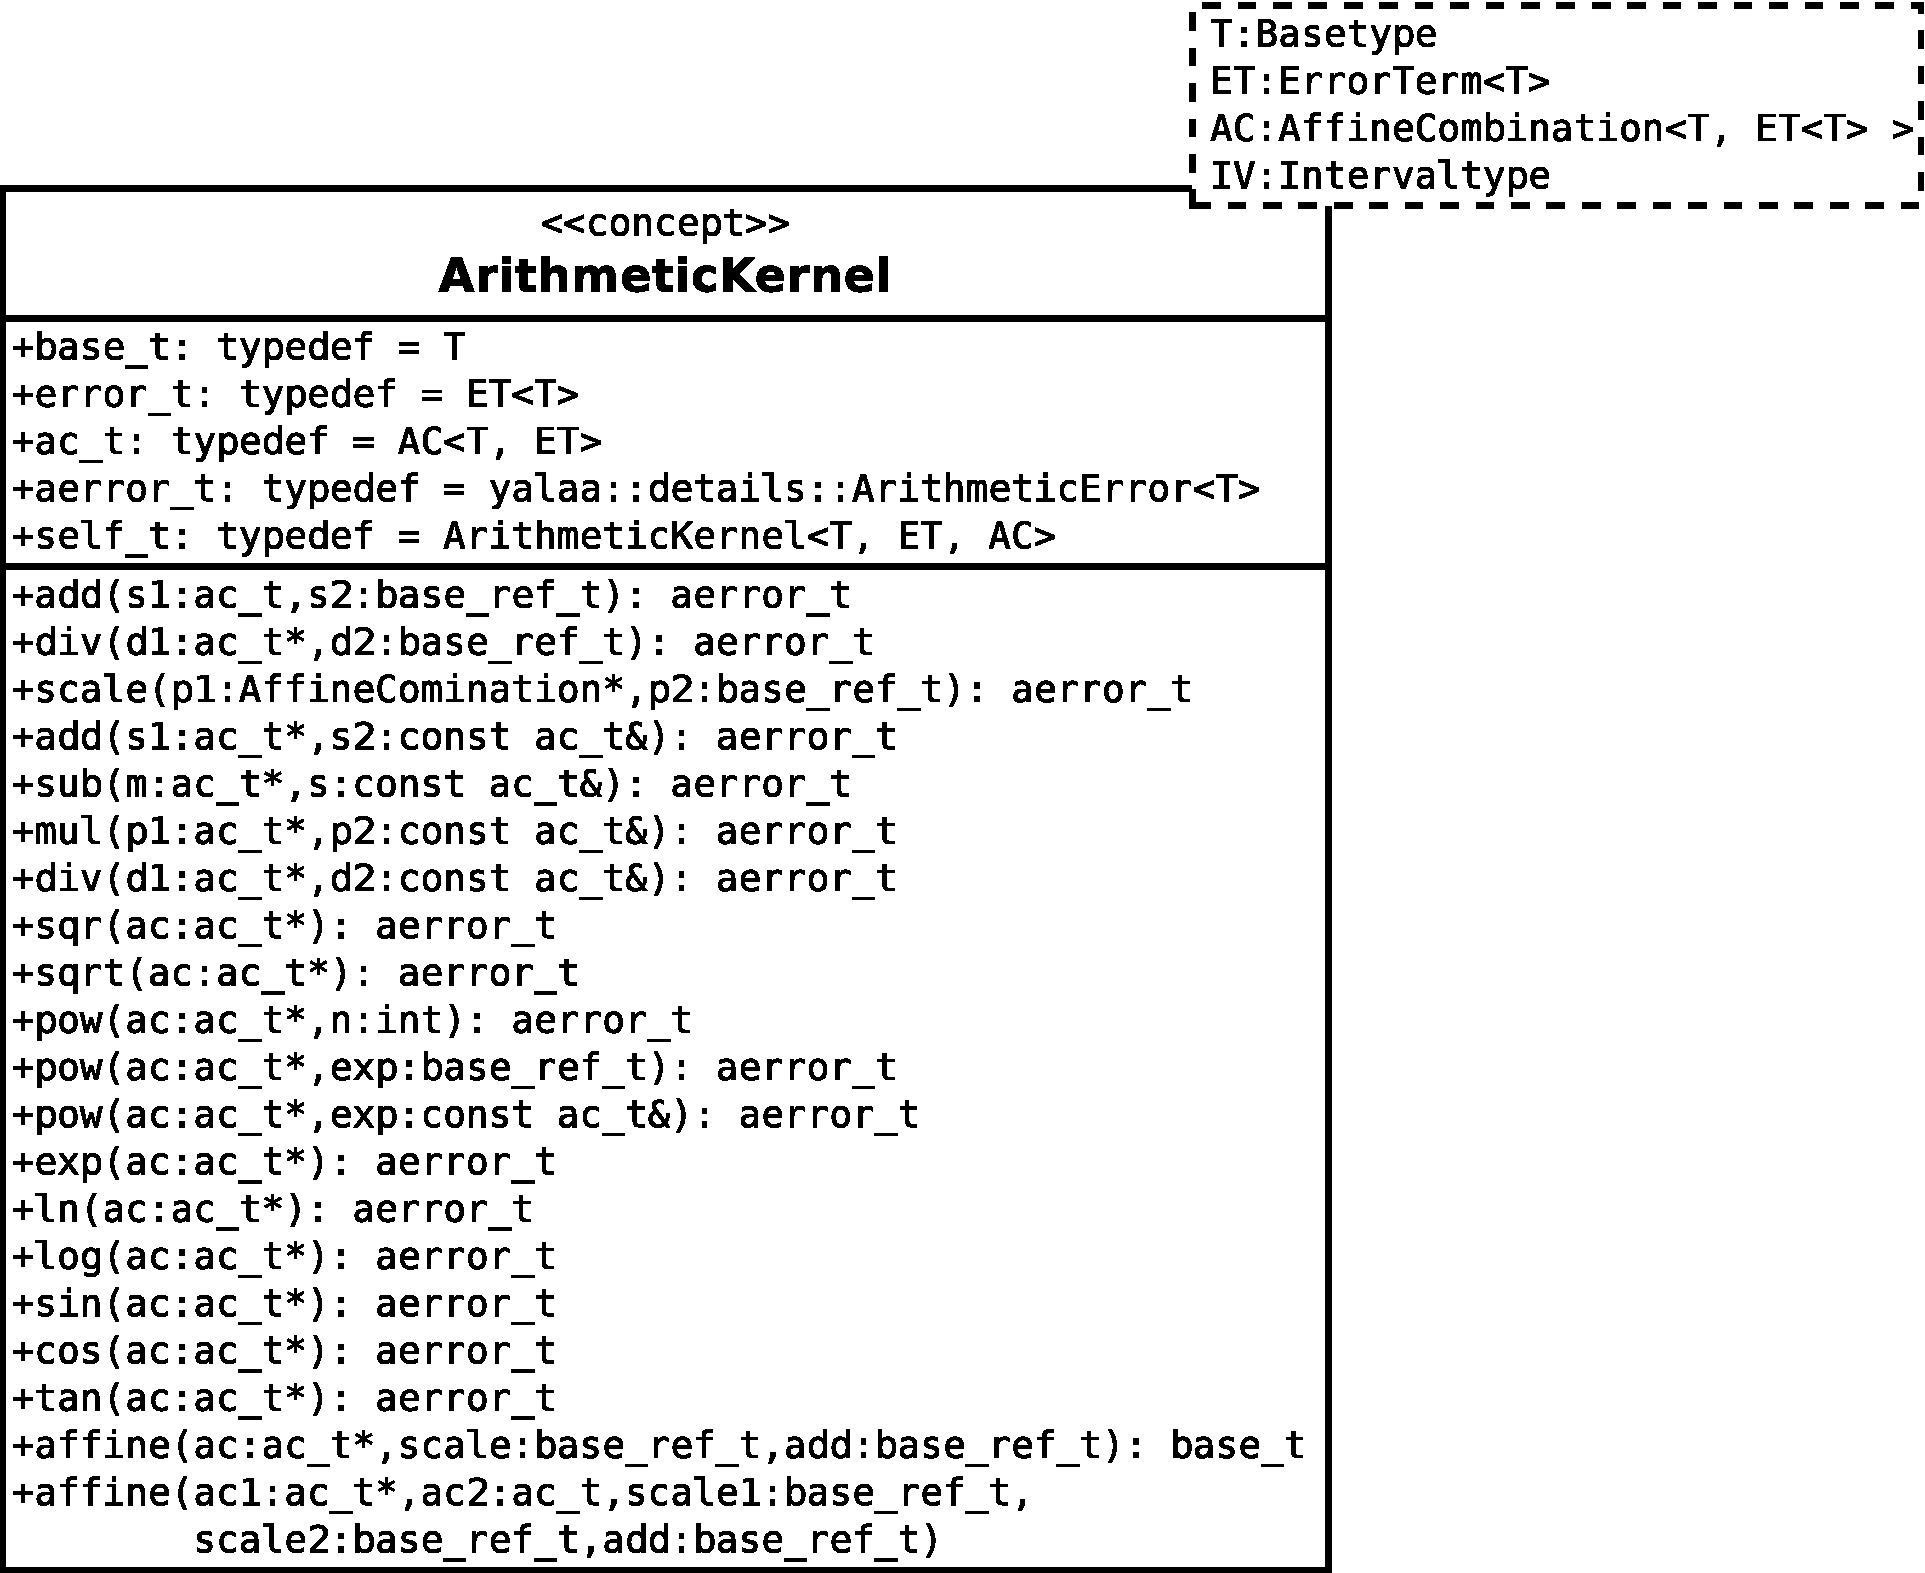
\includegraphics[width=0.5\textwidth]{arithmetickernel}
  \caption{Concept defining an ArithmeticKernel}
  \label{fig:arith_kernel}
\end{figure}
The arithmetic kernel is the core of \yalaa and carries out the actual
mathematical operations. This design ensures easy interchangeability of
operations. All operations are given in Fig. \ref{fig:arith_kernel}. All
operations work on a given affine combination, which is altered during
computation. However, they \emph{must not} add any new error terms to the
combination. Instead they deliver bounds of the occurring
errors to the caller through an \texttt{ArithmeticError<T>} object. New
noise terms are added through the \texttt{AffinePolicy}, which is described
later on. 

\paragraph{AffinePolicy}
\begin{figure}[h]
  \centering
  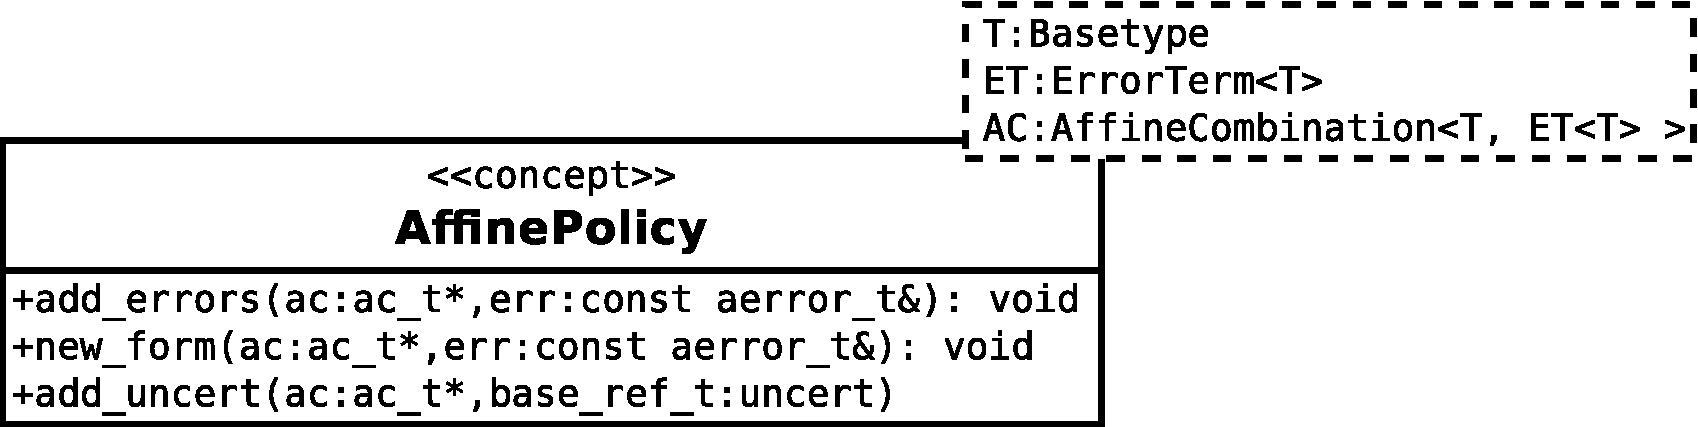
\includegraphics[width=0.5\textwidth]{affinepolicy}
  \caption{Concept defining an \texttt{AffinePolicy}}
  \label{fig:affine_policy}
\end{figure}
The \texttt{AffinePolicy} controls the way new affine noise symbols are
introduced. All operations are given in Fig. \ref{fig:affine_policy}. The
difference between the functions are subtle.  The \texttt{add\_errors}
function is called after performing an affine or non-affine combination. The
function is responsible for adding the rounding and/or approximation error to the
form.  In contrast \texttt{new\_form} is called if a new affine form is
created, i.e. a new partially unknown quantity is introduced into the
computation process. With \texttt{add\_uncert} an uncertainty is introduced
into the calculation process, this function is for example called if an affine
form is combined with an interval quantity.

\paragraph{ErrorPolicy}
\label{sec:errorpolicy}
\begin{figure}[h]
  \centering
  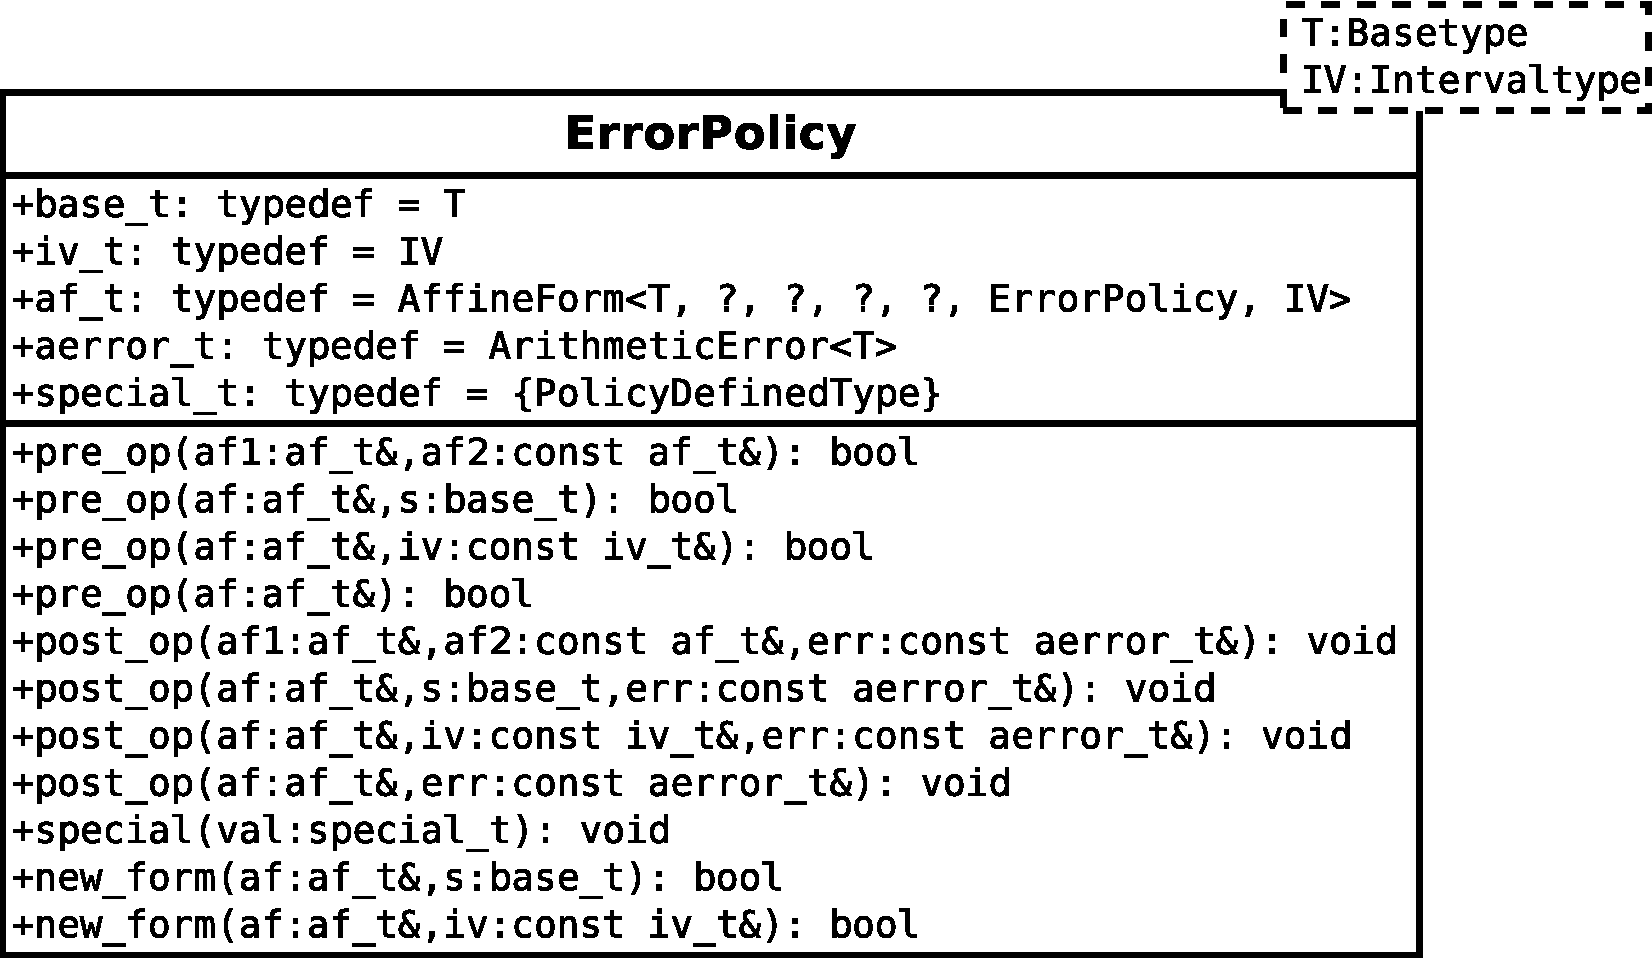
\includegraphics[width=0.7\textwidth]{errorpol}
  \caption{Concept defining an \texttt{ErrorPolicy}}
  \label{fig:error_policy}
\end{figure}
The \texttt{ErrorPolicy} is responsible for handling errors during the
computation process. These errors are propagated through the error flags of
the \texttt{ArithmeticError} class. Its methods are listed in
Fig. \ref{fig:error_policy}. The \texttt{pre\_op} functions are called prior
to performing an operation. If the arguments generate independent of the
concrete function a special form, the functions should return \texttt{false}
and modify its first argument accordingly. Then the calculation step is
skipped and the special form is returned. Otherwise, the regular
\texttt{ArithmeticKernel} operation is called and the resulting
\texttt{ArithmeticError} object is passed to the \texttt{post\_op}
operation. Once again, the \texttt{ErrorPolicy} should check whether to
generate an appropriate special form.


\subsection{Supplied Implementations}
\yalaa is delivered with some standard implementations for the above described
concepts. 
\paragraph{ErrorTerm}
The supplied standard implementation \texttt{ErrorTermImpl<T>} uses an
\texttt{unsigned long long}\footnote{According to C99 at least 64-bits wide}
and the \texttt{GCC}'s built-ins for atomic memory access. However, overflows
in the $\epsilon$'s are not handled. You should replace the default
implementation, if you need more than $2^{64}$ independent error terms.

\paragraph{AffineCombImpl}
The provided standard implementation \texttt{AffineCombImpl} uses a vector for
storing the error terms. (TODO: Spezielle Formen wie AF1, AF2, GQF,...)

\paragraph{Affine operations}
A standard implementation is supplied
in the file \texttt{affinecombopimpl.hpp}.

\paragraph{ArithmeticKernel}
\yalaa contains a complete kernel for AA which can work with the IEEE 754
floating-point types \texttt{float}, \texttt{double}, \texttt{long double}.
The implementation \texttt{ExactErrorFP} follows the approach described in
\cite{stolfi1997} where possible. However, the there described approximation
methods for non-affine operations are only applicable for strictly convex or
concave functions. For other functions (e.g. $\cos, \sin, \tan$) \yalaa uses a
Chebyshev interpolation based approach as outlined in
Sect. \ref{sec:chebysh-interp}. To ease reuse, we have split the
\texttt{ExactErrorFP} kernel into several components
(cf. Tab. \ref{tab:comp_arith_kernel}).
\begin{table}[h]
  \centering
  \begin{tabular}{lp{0.25\textwidth}p{0.5\textwidth}}
    \hline
    Name & Operations & Remarks\\
    \hline
    ExactErrorAffineFPf & \texttt{add, sub, scale, neg} & Affine operations with exact
    floating-point error calculation, \cite{stolfi1997}\\
    MinRangeBuiltInFP & \texttt{sqrt, inv} & Min-range, \cite{stolfi1997}\\
    MinRangeFP & \texttt{exp, ln} & Min-range, needs IA library, cf. \cite{stolfi1997}\\
    MultiplicationFP & \texttt{mul, sqr, pow} & Stolfi approach to
    multiplication, needs IA lib, \cite{stolfi1997}, Sect. \ref{sec:integ-power-funct}\\
    ChebyshevFP & \texttt{cos, sin, tan} & Chebyshev interpolation approach,
    needs IA lib, Sect. \ref{sec:chebysh-interp}\\
    \hline
    % ExactError & \emph{all} & Combination of \texttt{ExactErrorAff}, \texttt{MulOrig}
    % \texttt{MinRange}, \texttt{ChebyNonCC}, \texttt{div} via \texttt{mul} and \texttt{inv}\\
    % IVError & - & Interval arithmetic approach, !TODO!\\
    % PostError & - & COSY like approach, !TODO!\\
  \end{tabular}
  \caption{Components of the \texttt{ExactErrorFP} kernel}
  \label{tab:comp_arith_kernel}
\end{table}
% The \texttt{ExactError} kernel is basically an implementation of the original
% affine arithmetic, as proposed by its inventors de Figueiredo and Stolfi in
% \cite{stolfi1997}. They only consider approximations for non affine functions
% which are strictly convex or concave, so the trigonometric standard functions
% are not included in their approach. For computing these, the procedure
% described in !TODO! is used.

\paragraph{AffinePolicy}
\label{sec:affinepolicy}
The policy class \texttt{AF0} supplied with \yalaa mimics the behavior of the
original affine arithmetic as described in \cite{stolfi1997}. All policy
functions add the error with a new independent error symbol. 

\paragraph{ErrorPolicy}
\label{sec:errorpolicy-1}
Three implementations of the \texttt{ErrorPolicy} concept are supplied with
\yalaa: \texttt{ErrorPolStd}, \texttt{ErrorPolNone} and \texttt{ErrorPolDec}.
The \texttt{ErrorPolStd} resembles the approach described in \cite{stolfi1997}
and thus provides two special forms:
\begin{description}
  \item[\texttt{NONE}] No special value
  \item[\texttt{R}] Whole real line
  \item[\texttt{EMPTY}] Empty affine form
\end{description}
Tab. \ref{tab:errorpolstd_map} shows how the \texttt{ArithmeticError} flags
are mapped to these values and how they behave under combinations. As \yalaa
allows combination of affine forms with the scalars and intervals of the base
type, it is also necessary to \emph{their} special values. In general
\texttt{ErrorPolStd} uses the function \texttt{is\_special} of the respective
\texttt{base\_traits} specialization for checking if the operand is
valid. If it is not the outcome is \texttt{EMPTY}. Further, we provide a
specialization for floating-point base types handling $\pm \infty$
values and \texttt{NaN} separately. A $\pm \infty$ operand or an unbounded
interval generates \texttt{R} and \texttt{NaN} yields \texttt{EMPTY}.

In \texttt{ErrorPolNone} no error handling at all is done and
\texttt{ErrorPolDec} tries to provide the decorations concept of the upcoming
interval standard \cite{P1788022} for affine arithmetic. A detailed
description is given in \cite{yalaadeko}.
\begin{table}
  \centering
  \begin{tabular}{ll||l|lll}
    \hline
    Flag & Mapping & $\circ$ & \texttt{NONE} & \texttt{R} & \texttt{EMPTY} \\
    \hline
    \texttt{DISCONT} & \texttt{NONE} & \texttt{NONE}&  \texttt{NONE} &
    \texttt{R} & \texttt{EMPTY }\\
    \texttt{UNBOUND} & \texttt{R} & \texttt{R} & \texttt{R} & \texttt{R} & \texttt{EMPTY}\\
    \texttt{P\_D\_VIOL} & \texttt{NONE} & \texttt{EMPTY} & \texttt{EMPTY} &
    \texttt{EMPTY} & \texttt{EMPTY}\\
    \texttt{C\_D\_VIOL} & \texttt{EMPTY} & &\\
    \texttt{OVERFLOW} & \texttt{R} & & \\
    \texttt{ERROR} & \texttt{EMPTY} & &\\
    \hline
  \end{tabular}
  \caption{Mapping of ArithmeticError flags to ErrorPolStd special values and
    outcome of combinations of them}
  \label{tab:errorpolstd_map}
\end{table}

% \subsection{Elementary Functions}
% \label{sec:elementary-functions}
% The supported elementary functions are described in
% Tab. \ref{tab:elementary_functions}. Note that the behavior of all elementary
% functions\footnote{except square root} is not specified by IEEE754. In C99 the
% accuracy and handling of rounding modes is \emph{implementation defined} in
% the C99 math library is implementation defined for these functions.

% \begin{table}
%   \footnotesize
%   \centering
%   \begin{tabular}{lllll}
%     \hline
%     Function & Method & Domain & Impl. & Notes\\
%     \hline
%     $\cos{x}$ & TS & $(-\infty, \infty)$ & IA & \\
%     $\exp{x}$ & MR & $(-\infty, \infty)$ & IA &  \\
%     $\ln{x}$ & MR & $(0, \infty)$ & IA &  Negatives parts of input are
%     discarded, base $e$\\
%     $\log{x}$ & MR & $(0, \infty)$ & IA &  Negatives parts of input are
%     discarded, base 10\\
%     $\sin{x}$ & TS & $(-\infty, \infty)$ & IA & \\
%     $\sqrt{x}$ & MR & $[0,\infty)$ & FP & Negative parts of input are
%     discarded\\
%     $\tan{x}$ & TS & $(-\infty, \infty)$ & IA & Argument reduction to \\
%     \hline
%   \end{tabular}
%   \caption{Supported elementary functions and their implementation. The column
%     method denotes whether a min-range (MR) or a Taylor series approximation
%     (TS) is used. The impl. columns informs if an external interval library
%     (IA) is required or standard IEEE 754 floating-point arithmetic (FP)
%     suffices. Both columns apply to the provided double
%     implementation.}
%   \label{tab:elementary_functions}
% \end{table}

\appendix

\section{Function Implemention}
\label{sec:funct-impl}
This section briefly summarizes the concrete floating-point implementation for
some functions provided by the \yalaa built-in kernels.
\subsection{Chebyshev Interpolation}
\label{sec:chebysh-interp}
The min-range approximation for calculating affine approximations to
non-affine functions described in \cite{stolfi1997} is only applicable to
differentiable strict convex or concave functions. As \yalaa also supports
elementary functions not satisfying these requirements, namely the
trigonometric functions $\cos, \sin \tan$, another method is required. The
standard arithmetic kernels supplied with \yalaa use interpolation at the
Chebyshev nodes for this. Readers interested in the mathematical details
are referred to \cite{kearfott2010} and \cite{mason2003}.

The Chebyshev nodes $x_k$ are defined as
\[
x_k = \cos \left ( \frac{\pi (2k+1)}{2n+2} \right ), k=0...n
\]
and are at the zeros of the Chebyshev polynomials
\[
T_i(x) = \cos i \theta \mathrm{\ ,if\ } x = \cos \theta .
\]
A function $f: \iv{-1}{1} \rightarrow \Rz$ can approximated using the $n$-th degree
Chebyshev interpolant
\[
p_n(x) = \frac{ c_0}{ 2} + \sum \limits_{k=1}^n c_kT_k(x)
\]
with the Chebyshev coefficients
\[
c_i = \frac{2}{n+1} \sum \limits_{k=0}^n f(x_k)T_i(x_k) .
\]

For approximating a function on a general finite interval $\iv{a}{b}$ a linear
transformation to $\iv{-1}{1}$ is necessary. The new Chebyshev nodes
are obtained through the inverse transformation as
\[
x_k' = \frac{1}{2}\left ( (b-a)x_k + a + b \right )
\]
and thus the coefficients as
\[
c_i' = \frac{2}{n+1} \sum \limits_{k=0}^n f(x_k')T_i(x_k) .
\]
The new interpolant is 
\[
p_n(x) = \frac{c_0}{2} + \sum \limits_{k=0}^n c_k' T_k(x) 
\]
for $x \in \iv{-1}{1}$. We can transform any $x' \in \iv{a}{b}$ using a
linear transformation $t: \iv{a}{b} \rightarrow \iv{-1}{1}$ with
\[
t(x') = \left ( \frac{2x' - (a+b)}{b-a}\right) .
\]
The final polynomial for $x'$ is thus
\[
p_n(x') = \frac{c_0}{2} + \sum \limits_{k=0}^n c_k' T_k(\left ( \frac{2x' - (a+b)}{b-a}\right)) .
\]

Following \cite{stolfi1997} we are searching an affine operation of the form
$\alpha \aff x + \zeta \pm \delta$ over the domain $\x = \iv{a}{b}$ of $\aff x$.
This is a degree one polynomial, thus only the coefficients $c_0'$ and $c_1'$
are required. We calculate enclosures
\[
\ialpha = \frac{2 c_1'}{b-a}
\]
and
\[
\izeta = \frac{c_0'}{2} - \frac{a+b}{b-a}
\]
for $\alpha$ and $\zeta$ utilizing IA. The rounding error is shifted into the
error term $\delta$ using
\[
\delta = \frac 1 2 \left ( \left (\mathrm{len}(\aff x) + 1 \right )\wid \ialpha + \wid \izeta  +
  \wid R_1(\x) \right) 
\]
where $\mathrm{len}(\aff x)$ denotes the number of noise symbols in $\aff x$.
Then we can use the midpoints $\imid \ialpha$ and $\imid \izeta$ as $\alpha$ and
$\zeta$. A bound for $R_1(\x)$ can derived with Lagrange remainder's
formula\footnote{If a second derivative is available.}
\[
R_1(\x) = \frac{(\wid \x)^2 f^{(2)}(\x)}{16}
\]

% If the domain $\x$ is in the form $\iv{-a}{a}$, then the interpolating
% Chebyshev polynomial of an odd function is also odd. In this case all even
% coefficients $c_{2i}$ are zero \cite{!!!}. \yalaa can exploit this special
% case by using a second order remainder bound
% \[
% R_2(\x) = \frac{(\wid \x)^3 f^{(3)}(\x)}{192}
% \]
\textbf{!!!! Ueberarbeiten, so wird es nicht gemacht !!!!}
The final result $\aff{x'}$ of the operation can determined by using the
affine transformation
\[
\begin{array}{ll}
  x'_0 &= \alpha x_0 + \zeta\\
  x'_i &= \alpha x'_i   
\end{array}
\]
The occurring rounding errors are also shifted into $\delta$, which is added
as new error term $\delta \epsilon_k$, where $\epsilon_k$ is a new independent
symbolic noise variable. 
%TODO: Fehlerheuristik, wann ist es sinnvoll die Range [a,b] zu erweitern. 

\subsection{Integer Power-Function}
\label{sec:integ-power-funct}
The integer power function $\pow(\aff x, n)$ for positive integers $n$. Using
the binomial coefficients we can derive the formula
\[
\begin{array}{lll}
  \aff{x}^n &=& \left ( x_0 + \sum \limits_{i=1}^m x_i\epsilon_i
  \right )\\
  & =& x_0^n + nx_0^{n-1} \left ( \sum \limits_{i=1}^mx_i\epsilon_i \right )+\\
  &&
  {n \choose 2}x_0^{n-2} \left (\sum \limits_{i=1}^m x_i\epsilon_i \right )^2 + {n \choose
    3}x_0^{n-3} \left (\sum \limits_{i=1}^m x_i\epsilon_i \right )^3 + ... +
  \left( \sum \limits_{i=1}^m x_i\epsilon_i \right )^n\\
\end{array}
\]
The first two terms of the sum are the affine part of the power function.
Following the affine multiplication routine by de Figueiredo and Stolfi
\cite{stolfi1997} the these terms are directly used for our affine
approximation. The non linear terms are enclosed by a new error term.
Let
\[
\rad \aff x = \sum \limits_{i=1}^m |x_i|
\]
so we get the error as
\[
e = {n \choose k} (\rad \aff x)^k .
\]
We split the error into an unsigned part $e^+$ for all terms with an even $k$
and a signed $e^\pm$ one for all odd terms. The final error
\[
e = \frac 1 2 e^+ + e^\pm
\]
is then added with a new noise symbol to the result. Finally the central value
is adjusted by $\frac 1 2 e^+$. 

% \section{Taylor Series Expansion}
% \label{sec:taylor-series}
% The min-range approximation (Sect. \ref{sec:min-range-appr}) is only
% applicable if the function is twice continuously differentiable and strictly
% convex or concave\footnote{In the domain of the considered affine form.}.  For
% non convex or concave functions in $\mathcal{C}^2$ an affine approximation
% $f^a(x) = \alpha x + \zeta \pm \delta$ can be retrieved using a Taylor series
% expansion.

% Let $\aff x$ denote the considered affine form, $\x \in \IRz$ its
% domain and $f \in \mathcal{C}^2\iv{\ul \x}{\ol \x}$ a function. Using Taylor's
% theorem we can rewrite $f$ as
% \begin{equation}
%   f(x) = f(a) + f'(a)(x-a) + R_1(x)
%   \label{eq:taylor_poly}
% \end{equation}
% with the Lagrange remainder
% \begin{equation}
%   R_1(x) = \frac{f''(\xi)}{2}(x-a)^2
% \end{equation}
% for some $\xi$ between $x$ and $a$. If we choose an expansion point inside
% $\x$ for example $a = \imid \x$, we can retrieve bounds for $R_1(x)$ with IA by
% replacing $\xi$ and $x$ by its bounds $\x$. This bound is shifted into the
% error term $\delta$ of our approximation. According to \eqref{eq:taylor_poly}
% slope $\alpha$ of $f^a(x)$ is $f'(a)$ and the independent term $\zeta$ is
% $f(a) - \alpha a$.

% In general we cannot determine values for $f'(a)$ and $f(a)$ exactly. However,
% we can retrieve verified bounds with IA and thus compute enclosures $\ialpha,
% \izeta \in \IRz$ with $\alpha \in \ialpha$ and $\zeta \in \izeta$. We shift
% the rounding error in the error term $\delta$ of our approximation using
% \[
% \delta = \frac 1 2 (\wid \ialpha + \wid \izeta  + \wid R_1(\x))
% \]
% Using the midpoints we get $\tilde \alpha = \imid \ialpha$ and
% $\tilde \zeta = \imid \izeta$. Then we apply the final affine approximation
% \begin{equation}
%   f^a(x) = \tilde \alpha x + \tilde \zeta \pm \delta
% \end{equation}
% to the affine form $\aff x$ as described in Sect. \ref{TODO}.



\bibliography{references}   % name your BibTeX data base
\bibliographystyle{plain}

\end{document}


%%% Local Variables: 
%%% mode: latex
%%% TeX-master: t
%%% End: 
